\section{Mass Resolution and Scale}
\label{sec:mass_res}

The mass resolution of heavy resonances is a crucial point of the analysis, since its outcome enters in the signal model definition. Its estimation follows two steps: a data-MC comparison, and a MC-only study.
The first step consists in the comparison between data and DY MC for the resolution and mean value of the invariant mass distribution of the electron pairs passing the HEEP ID at the Z peak (80 GeV $<M_{ee}<$ 100 GeV).
The distributions are fitted using a Breit-Wigner (B-W) function (whose parameters are fixed to the PDG values of the Z boson) convoluted with a double-sided crystal ball function (dCB) (which is defined as a Gaussian core connected with two power-law functions on both sides).
The $\sigma$ parameter from the dCB function is then compared between data an MC in different $\eta$-categories. For BB category both electrons are required to be in the ECAL barrel. For BE category one electron is required to be in the ECAL barrel, and the other one in one of the ECAL endcaps.
Fit results for data and MC in 2016 (2017) are shown in Figure \ref{fig:data_MC_peak_2016} (\ref{fig:data_MC_peak_2017}).

The $\sigma_{MC}$ of the dCB from the fit to the MC distribution is subtracted in quadrature by the $\sigma_{data}$ coming from the fit to the data, and defining the $\sigma_{extra}$ through the relation: $\sigma_{extra}=\sqrt{\sigma_{data}^{2} - \sigma_{MC}^{2}}$.
In Table \ref{tab:extra} the results for the $\sigma_{extra}$ are shown for the different categories for 2016 and 2017.
Note that the numbers in Table \ref{tab:extra} are presented in percentage [\%] of the Z peak mass value (it is 91.1876 GeV for $M_{Z}$ DPG ). The quoted mean values are the ones of the dCB function used to fit the mass spectra after convolution with the B-W function. For 2017 the official EGamma energy scale and smearing is applied for data and MC, therefore the mean value difference between data and MC in 2017 is much smaller than that in 2016 and for the $\sigma_{extra}$ which is 0 in 2017 because of the larger $\sigma_{MC}$ than $\sigma_{data}$.

\begin{figure}[ht]
  \begin{center}
    \begin{tabular}{cc}
      \includegraphics[width=0.48\textwidth]{figures/Zprime/2016/mass_resolution/h_mee_data_BB_2016_Moriond17.pdf} &
      \includegraphics[width=0.48\textwidth]{figures/Zprime/2016/mass_resolution/h_mee_data_BE_2016_Moriond17.pdf} \\
      \includegraphics[width=0.48\textwidth]{figures/Zprime/2016/mass_resolution/h_mee_MC_BB_2016_Moriond17.pdf} &
      \includegraphics[width=0.48\textwidth]{figures/Zprime/2016/mass_resolution/h_mee_MC_BE_2016_Moriond17.pdf}
    \end{tabular}
    \caption{The distributions of dielectron invariant masses at the Z peak in data (top) and MC (bottom) for the BB (left) and BE (right) regions in 2016 \cite{CMS-AN-2016-404}.
    \label{fig:data_MC_peak_2016}}
  \end{center}
\end{figure}

\begin{figure}[ht]
  \begin{center}
    \begin{tabular}{cc}
      \includegraphics[width=0.48\textwidth]{figures/Zprime/2017/mass_resolution/data_BB_RunBCDEF} &
      \includegraphics[width=0.48\textwidth]{figures/Zprime/2017/mass_resolution/data_BE_RunBCDEF} \\
      \includegraphics[width=0.48\textwidth]{figures/Zprime/2017/mass_resolution/mc_BB} &
      \includegraphics[width=0.48\textwidth]{figures/Zprime/2017/mass_resolution/mc_BE}
    \end{tabular}
    \caption{The distributions of dielectron invariant masses at the Z peak in data (top) and MC (bottom) for the BB (left) and BE (right) regions in 2017.
    \label{fig:data_MC_peak_2017}}
  \end{center}
\end{figure}



\begin{table}[htb]
\begin{center}
\begin{tabular}{cccccc}
\hline
Year &Category            & $\frac{\Delta M}{M} [\%]$ & $\sigma_{data}$ [\%] & $\sigma_{MC}$ [\%] & $\sigma_{extra}$ [\%] \\ \hline
\multirow{2}{*}{2016}     &BB       & -0.19 $\pm$ 0.02          & 1.45 $\pm$ 0.00      & 1.20 $\pm$ 0.03    & 0.81 $\pm$ 0.04  \\
                          &BE       & -0.40 $\pm$ 0.02          & 2.49 $\pm$ 0.01      & 2.15 $\pm$ 0.03    & 1.26 $\pm$ 0.05  \\ \hline
\multirow{2}{*}{2017}     &BB       & 0.04 $\pm$ 0.01           & 1.63 $\pm$ 0.01      & 1.74 $\pm$ 0.01    & 0 $\pm$ 0 \\
                          &BE       & -0.03 $\pm$ 0.00          & 2.91 $\pm$ 0.00      & 2.93 $\pm$ 0.00    & 0 $\pm$ 0 \\ \hline
\end{tabular}
\caption{The results of scale shift $\frac{\Delta M}{M}$  between data and MC, as well as the $\sigma_{extra}$ parameters per category. \label{tab:extra}}
\end{center}
\end{table}
\medskip


In 2017 we also checked mass scale and resolution for data and MC as a function of \et, energy and $\eta$ of electron using the method explained above.
Results are shown from Figure \ref{fig:data_MC_Et_E_BB} to \ref{fig:data_MC_eta_BB_BE}. In all \et and  $\eta$ ranges, the data and MC show good agreement.
The energy scale at high \et is validated to within 2\% for barrel electrons and 1\% for endcap elections.

\begin{figure}[ht]
  \begin{center}
    \begin{tabular}{cc}
      \includegraphics[width=0.48\textwidth]{figures/Zprime/2017/mass_resolution/scale_check/h_led_Et_Mee_BB_scale} &
      \includegraphics[width=0.48\textwidth]{figures/Zprime/2017/mass_resolution/scale_check/h_led_Et_Mee_BB_resolution} \\
      \includegraphics[width=0.48\textwidth]{figures/Zprime/2017/mass_resolution/scale_check/h_led_E_Mee_BB_scale} &
      \includegraphics[width=0.48\textwidth]{figures/Zprime/2017/mass_resolution/scale_check/h_led_E_Mee_BB_resolution}
    \end{tabular}
    \caption{The mean (left) and sigma (right) values of dCB as the function of \et (top) and energy (bottom) of leading electron for barrel-barrel channel.
    \label{fig:data_MC_Et_E_BB}}
  \end{center}
\end{figure}

\begin{figure}[ht]
  \begin{center}
    \begin{tabular}{cc}
      \includegraphics[width=0.48\textwidth]{figures/Zprime/2017/mass_resolution/scale_check/h_endcap_Et_Mee_BE_scale} &
      \includegraphics[width=0.48\textwidth]{figures/Zprime/2017/mass_resolution/scale_check/h_endcap_Et_Mee_BE_resolution} \\
      \includegraphics[width=0.48\textwidth]{figures/Zprime/2017/mass_resolution/scale_check/h_endcap_E_Mee_BE_scale} &
      \includegraphics[width=0.48\textwidth]{figures/Zprime/2017/mass_resolution/scale_check/h_endcap_E_Mee_BE_resolution}
    \end{tabular}
    \caption{The mean (left) and sigma (right) values of dCB as the function of \et (top) and energy (bottom) of endcap electron for barrel-endcap channel.
    \label{fig:data_MC_Et_E_BE}}
  \end{center}
\end{figure}

\begin{figure}[ht]
  \begin{center}
    \begin{tabular}{cc}
      \includegraphics[width=0.48\textwidth]{figures/Zprime/2017/mass_resolution/scale_check/h_float_eta_Mee_BB_scale} &
      \includegraphics[width=0.48\textwidth]{figures/Zprime/2017/mass_resolution/scale_check/h_float_eta_Mee_BB_resolution} \\
      \includegraphics[width=0.48\textwidth]{figures/Zprime/2017/mass_resolution/scale_check/h_endcap_eta_Mee_BE_scale} &
      \includegraphics[width=0.48\textwidth]{figures/Zprime/2017/mass_resolution/scale_check/h_endcap_eta_Mee_BE_resolution}
    \end{tabular}
    \caption{The mean (left) and sigma (right) values of dCB as the function of $\eta$ of second electron (the first electron is asked to have $|\eta|<0.5$) for barrel-barrel (top) and barrel-endcap (bottom) channels.
    \label{fig:data_MC_eta_BB_BE}}
  \end{center}
\end{figure}





The second step of the study is based on MC only.
In particular, the mass resolution has been studied as a function of the generated invariant mass of the electron pair $m_{gen}$.
In order to maximise the statistics, different mass bin (from 200-5000 GeV) DY samples are used.

For each bin of the generated invariant mass $m_{gen}$, the distribution of the difference between the reconstructed and the generated invariant mass,
divided for the generated invariant mass is analyzed.
Defining a variable $resolution =\frac{m_{reco}-m_{gen}}{m_{gen}}$, its distribution is then acquired as a function of $m_{gen}$, and a maximum-likelihood
fit to the distribution in each mass bin is performed using a ``Cruijff function'' (which is defined as a Gaussian core connected with an exponential tail on each side) in 2016. While in 2017, the dCB function is used for the fit because it is found that the Cruijff is not able to correctly describe the invariant mass shape at very high mass due to electron saturation effects \footnote{When the deposite energy in single ECAL crystal is very high, the electric readout will be saturated because of limited dynamic range. See more details in Appendix \ref{app:Saturation}}.
Finally, the sigma parameter ($\sigma_{fit}$) of the fit function is added in quadrature with the $\sigma_{extra}$ coming from the first step of the study.

The fitted parameters are studied in their behaviour versus the corresponding generated mass and an analytic parametrisation is provided and used
as an input for the limit setting procedure (more details are given in appendix \ref{app:_mas_res}).
Results of mass resolution for the BB and BE regions are shown in Figure \ref{fig:resolution}.

\begin{figure}[ht]
\centering
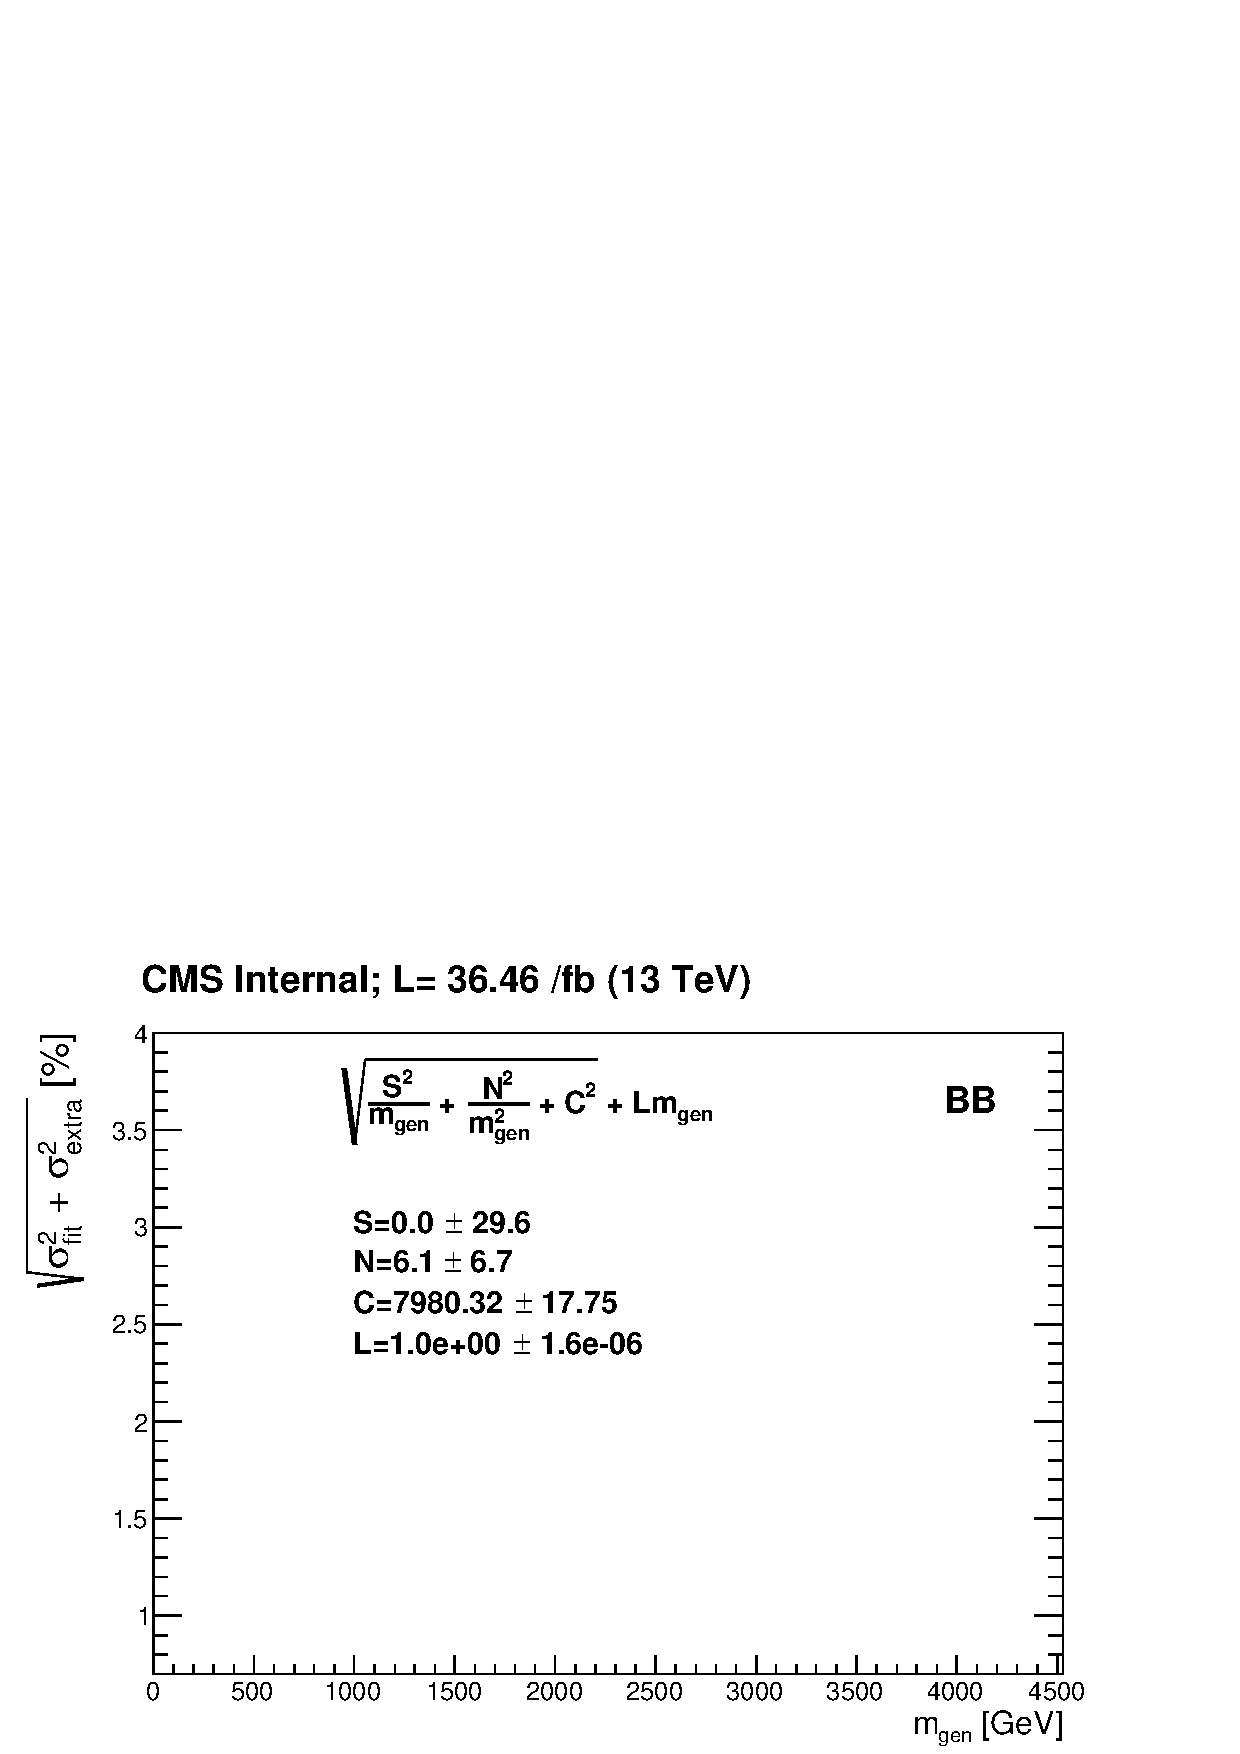
\includegraphics[width=0.48\textwidth]{figures/Zprime/2016/mass_resolution/resolution_BB.pdf}
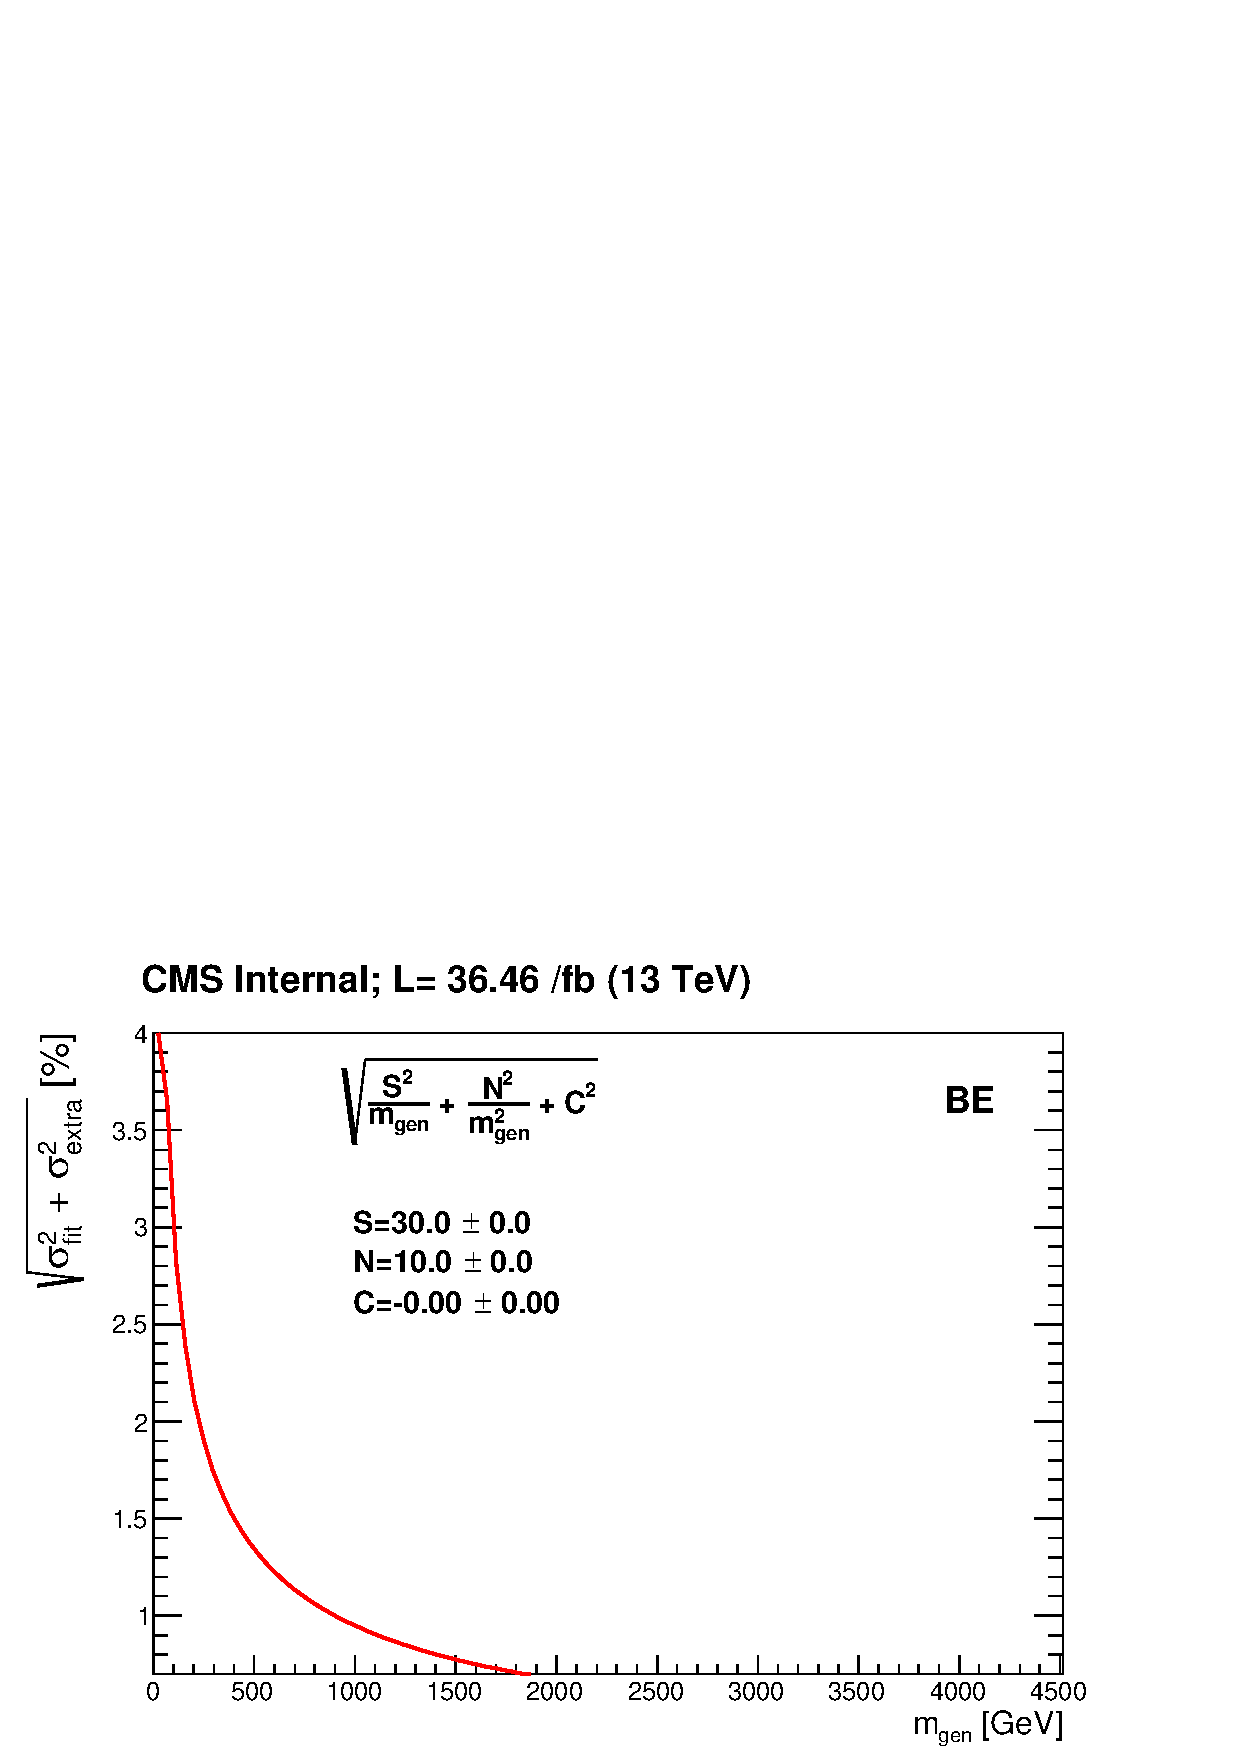
\includegraphics[width=0.48\textwidth]{figures/Zprime/2016/mass_resolution/resolution_BE.pdf}
\includegraphics[width=0.48\textwidth]{figures/Zprime/2017/mass_resolution/High_Mass/BB_sigma}
\includegraphics[width=0.48\textwidth]{figures/Zprime/2017/mass_resolution/High_Mass/BE_sigma}
\caption{The mass resolutions ($\sigma_{fit}$) as a function of generated Z boson mass for BB (left) and BE (right) regions in 2016 (top) \cite{CMS-AN-2016-404} and 2017 (bottom).
 \label{fig:resolution}}
\end{figure}

%The binning of the $x-$axis is chosen in order to have a reasonable amount of statistics for each range of $m_{ee}$ and ensure in this way a good quality, in terms
%of reduced $\chi^{2}$, of the performed fits.
%Some fit results are shown in Fig. \ref{fig:fits_BB} for the BB region, corresponding from left to right to the first bin of the mass resolution plot, the minimum of the mass resolution (encountered around $\approx$~1 TeV), and the last bin.
%\begin{figure}[ht]
%\centering
%\includegraphics[width=0.3\textwidth]{fig/mass_resolution/h_resolution_BB_1_bin_0.pdf}
%\includegraphics[width=0.3\textwidth]{fig/mass_resolution/h_resolution_BB_5_bin_4.pdf}
%\includegraphics[width=0.3\textwidth]{fig/mass_resolution/h_resolution_BB_19_bin_11.pdf}
%\caption{Fit results for the mass resolution, in the BB region.
% \label{fig:fits_BB}}
%\end{figure}

%With the same logic, some fit results are shown in Fig. \ref{fig:fits_BE} for the BE region, corresponding from left to right to the minimum of the mass resolution (encountered between 1-2 TeV), and the last two bins.
%
%\begin{figure}[ht]
%\centering
%\includegraphics[width=0.3\textwidth]{fig/mass_resolution/h_resolution_BE_7_bin_5.pdf}
%\includegraphics[width=0.3\textwidth]{fig/mass_resolution/h_resolution_BE_13_bin_7.pdf}
%\includegraphics[width=0.3\textwidth]{fig/mass_resolution/h_resolution_BE_17_bin_8.pdf}
%\caption{Fit results for the mass resolution, in the BE region.
% \label{fig:fits_BE}}
%\end{figure}

In the BB region there is a small linear rise in the mass resolution starting around $\approx$ 1.5 TeV. The effect has been already studied in \cite{CMS-AN-2015-222} and it is due to leakage of the electromagnetic ECAL shower in the HCAL subdetector which worsen in this way the energy reconstruction driven by the ECAL detector.
In fact, the effect of the leakage in the HCAL subdetector is visible as an increase in the $H/E$ variable, which is the ratio between the energy in the HCAL over the energy contained in the ECAL detector around the electron direction. For the increase of mass resolution from 4.5 TeV to 5 TeV in BB region is because the saturation effect becomes significant.
%The mean of $H_1/E_1 + H_2/E_2$ is shown in Figure \ref{fig:hoe}, where $1$ and $2$ label the first and the second electron, as a function of the invariant mass $m_{gen}$. Only in the BB region there is an increase at high mass, while in the BE region it stays rather flat.

%\begin{figure}[ht]
%\centering
%\includegraphics[width=0.48\textwidth]{fig/mass_resolution/HoverE_BB.pdf}
%\includegraphics[width=0.48\textwidth]{fig/mass_resolution/HoverE_BE.pdf}
%\caption{Mean of $H_1/E_1 + H_2/E_2$ as a function of the generated invariant mass for the BB region (left) and BE (right) channel.
% \label{fig:hoe}}
%\end{figure}

%It is also possible to quantify the leakage in the HCAL subdetector considering the behavior of $(H_1 + H_2)/(E_1 + E_2)$, where again $1$ and $2$ label the first and the second electron, as a function of the invariant mass $m_{gen}$. The behavior is very similar to the one of the other possible variable $H_1/E_1 + H_2/E_2$, apart from the absolute y-axis scale (See Figure \ref{fig:hoe_tot}).

%\begin{figure}[ht]
%\centering
%\includegraphics[width=0.48\textwidth]{fig/mass_resolution/HTotoverETot_BB.pdf}
%\includegraphics[width=0.48\textwidth]{fig/mass_resolution/HTotoverETot_BE.pdf}
%\caption{Mean of $(H_1 + H_2)/(E_1 + E_2)$ as a function of the generated invariant mass for the BB region (left) and BE (right) channel.
% \label{fig:hoe_tot}}
%\end{figure}

%As a cross-check in support of the HCAL leakage explanation, it is possible to show that the $\eta$ distribution for electrons in the ECAL barrel is different for the BB
%and BE category: in particular the electrons belonging to the BB category can be both low-$\eta$ and high-$\eta$ electrons, while in BE category there are mostly high-$\eta$
%electrons (see Figure \ref{fig:eta_check}.)

%\begin{figure}[!htbp]
%\begin{center}
%\includegraphics[width=0.48\textwidth]{fig/mass_resolution/eta_distributions.png}
%\end{center}
%\caption{$|\eta|$ distribution for the electrons falling in the ECAL barrel for BB category and BE category}
%\label{fig:eta_check}
%\end{figure}


%As a cross-check in support of the HCAL leakage explanation, the reconstructed energy is corrected, simply adding linearly the $H/E$ energetic fraction, without taking into account extra calibration coefficients. With this simple implementation, the resolution in the BB category appear much flatter at high $m_{gen}$ and in this configuration the rise is less pronounced, consisting in a 0.1 \% effect (See fig. \ref{fig:resolution_recover}).
%
%\begin{figure}[ht]
%\centering
%\includegraphics[width=0.6\textwidth]{fig/mass_resolution/resolution_h_recover_BB.pdf}
%\caption{Mass resolution as a function of the generated invariant mass for the BB category. The reconstructed energy is corrected to take into account the leakage in the HCAL subdetector.
% \label{fig:resolution_recover}}
%\end{figure}
%
%
%
%Finally, it is interesting to compare the obtained mass resolution plots with the ones that could be obtained using the raw-supercluster energy as reconstructed energy,
%so taking away the additional corrections applied in order to match the Z peak in data and MC.
%The comparison between those 2 possibilities (with the full reconstructed energy and using only the raw energy) are shown in Fig. \ref{fig:comparison_res}.
%
%\begin{figure}[ht]
%\centering
%\includegraphics[width=0.48\textwidth]{fig/mass_resolution/resolution_BB_comparison.png}
%\includegraphics[width=0.48\textwidth]{fig/mass_resolution/resolution_BE_comparison.png}
%\caption{Comparison between the mass resolution obtained using the full reconstructed energy (black points) and the raw-supercluster energy (red points) as a function of the generated invariant mass for the BB region (left) and BE (right) channel.
% \label{fig:comparison_res}}
%\end{figure}
%
%The comparison shows that in both regions, at high mass, the two different configurations tend to converge and, apart from some fluctations they show similar behavior.
\medskip
Also the mass scale of the ECAL detector has been studied as a function of the generated invariant mass of the electron pair $m_{gen}$, using the same generated samples taken into account for the mass resolution determination.

Defining the mass scale variable as $scale =\frac{m_{reco}}{m_{gen}}$, where $m_{gen}$ is the generated invariant mass, $m_{reco}$ is the reconstructed invariant mass. From the $resolution$ variable defined above it is easy to see that $scale= \frac{m_{reco}}{m_{gen}}= 1 + resolution$.
Therefore, the mass scale is taken from the mean parameter of the function used to fit the $resolution$ distribution and simply adding the unity to it. Besides, the error on the mean parameter is taken accordingly.

Results of mass scale for the BB and BE regions are shown in Figure \ref{fig:scale}.

\begin{figure}[ht]
\centering
\includegraphics[width=0.48\textwidth]{figures/Zprime/2016/mass_resolution/scale_BB.pdf}
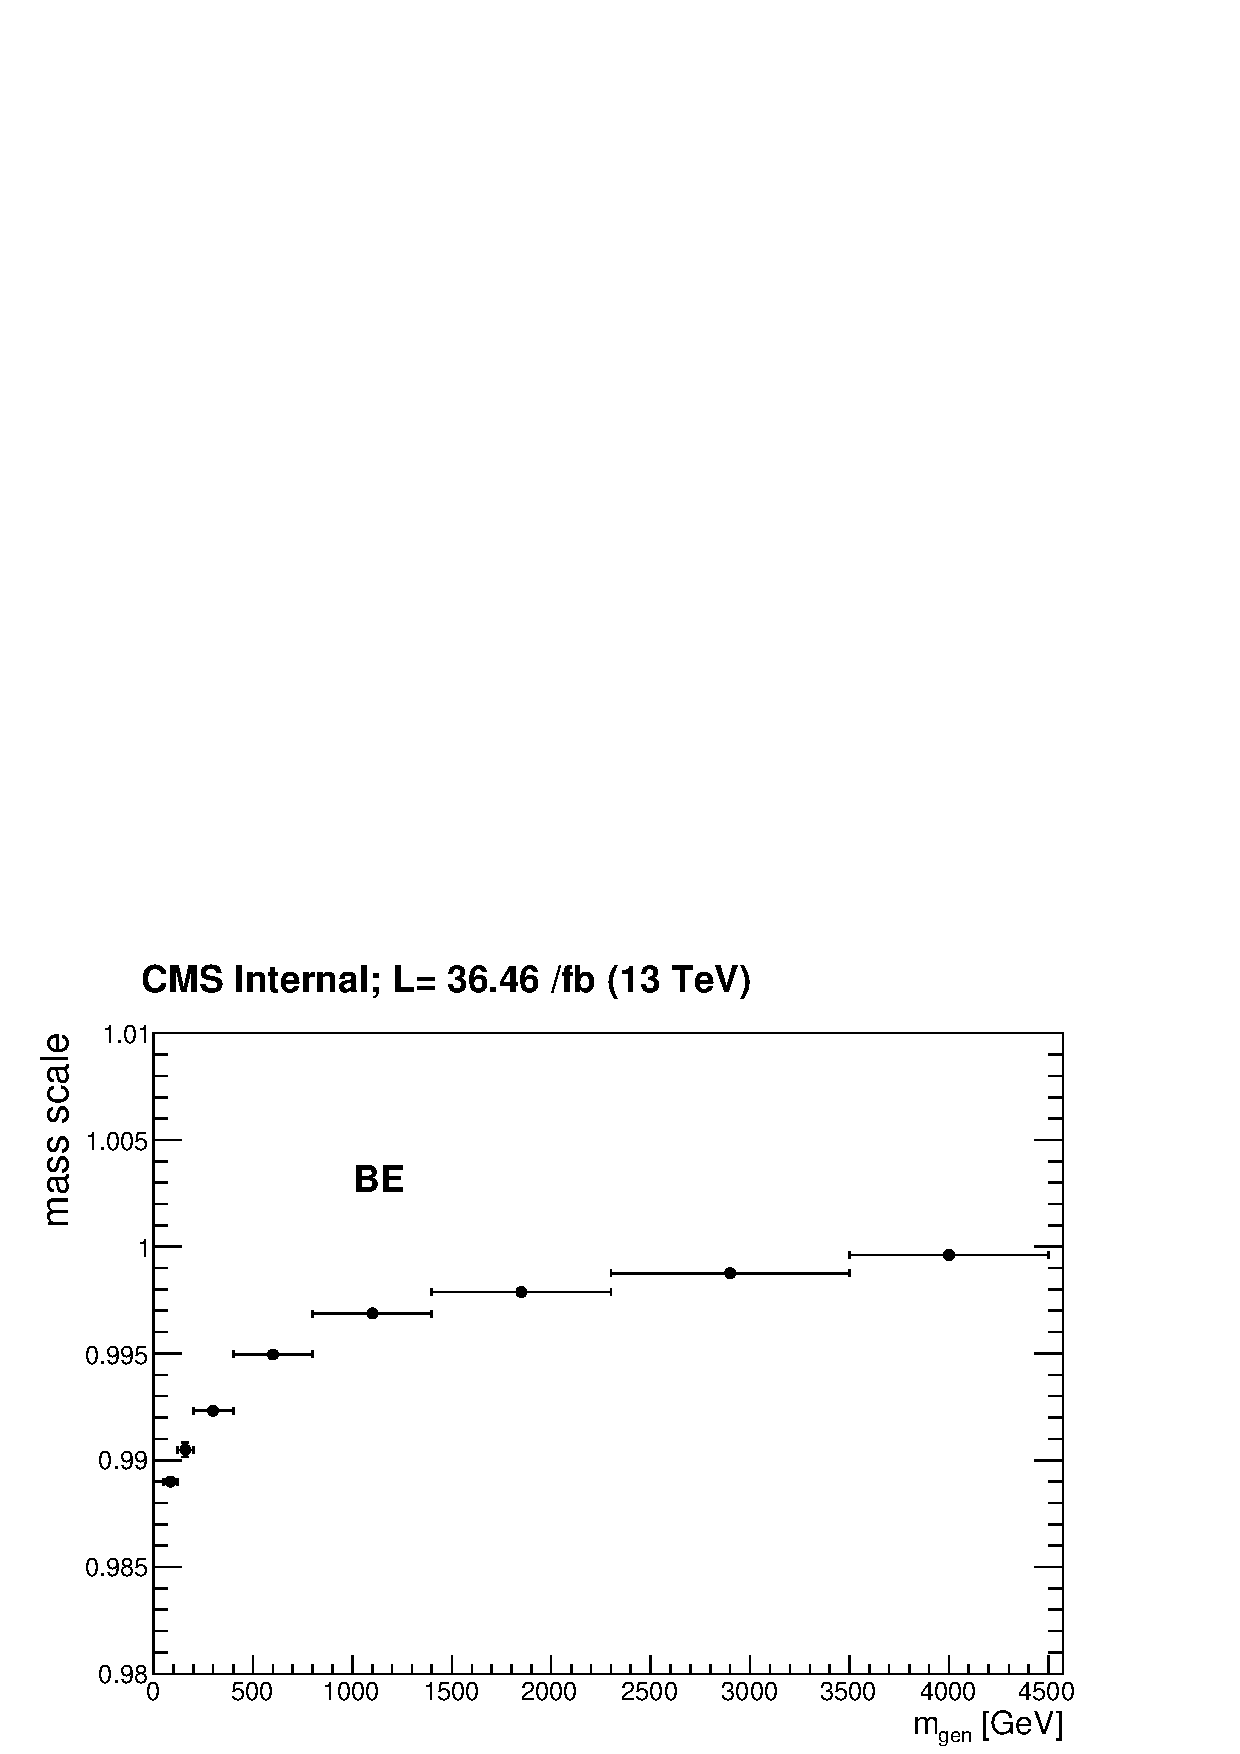
\includegraphics[width=0.48\textwidth]{figures/Zprime/2016/mass_resolution/scale_BE.pdf}
\includegraphics[width=0.48\textwidth]{figures/Zprime/2017/mass_resolution/High_Mass/BB_mean}
\includegraphics[width=0.48\textwidth]{figures/Zprime/2017/mass_resolution/High_Mass/BE_mean}
\caption{The mass scales as a function of generated Z boson mass for BB (left) and BE (right) regions in 2016 (top) \cite{CMS-AN-2016-404} and 2017 (bottom).
 \label{fig:scale}}
\end{figure}

In the BB region there is a drop in the mass scale parameter starting around $\approx$ 1 TeV ($\approx$ 0.5 \% effect), which is the counterpart of the rise observed in the mass resolution, and is again due to leakage of a small part of the high-energetic electromagnetic shower in the HCAL subdetector.
